\documentclass{beamer}
\usepackage[french]{babel}
\usepackage{hyperref}
\usepackage{graphicx}
\usepackage{amsmath,amssymb}
\usepackage{tabularx}
\usepackage{booktabs}
\usepackage[compatibility=false]{caption}
\usepackage[toc,page]{appendix}
\usepackage{minted}

\makeatletter
  \def\beamer@calltheme#1#2#3{%
    \def\beamer@themelist{#2}
    \@for\beamer@themename:=\beamer@themelist\do
    {\usepackage[{#1}]{\beamer@themelocation/#3\beamer@themename}}}

  \def\usefolder#1{
    \def\beamer@themelocation{#1}
  }
  \def\beamer@themelocation{}


\newcolumntype{Y}{>{\centering\arraybackslash}X}

\usefolder{../theme}
\usetheme[numbering=fraction,block=fill,progressbar=frametitle]{metropolis} %Use metropolis theme

\definecolor{bg}{rgb}{0.95,0.95,0.95}
\setminted{bgcolor=bg,fontsize=\scriptsize,autogobble,mathescape,breaklines,tabsize=2}
\setmintedinline{breaklines,autogobble,fontsize=\scriptsize}

\begin{document}

\title[C++]{Introduction à la programmation en C++}
\author[nicolas.audebert@onera.fr]{Nicolas Audebert}
\setmainfont{Fira Sans}


\AtBeginSection[]{
  \begin{frame}{Plan de la séance}
  \small \tableofcontents[currentsection]
  \end{frame}
}

\subtitle{Préliminaires}
\date{14 septembre 2018}
\maketitle

\section{Introduction}

\begin{frame}{Avant toute chose}
  \begin{block}{Supports de cours}
  \begin{itemize}
    \item Site du cours : {\small \url{http://imagine.enpc.fr/~monasse/Info/}}\\
  	\item Planches : {\small \url{https://nicolas.audebert.at/teaching/}}
  	\item Le polycopié \og La programmation pour les élèves-ingénieurs \fg
  \end{itemize}
  \end{block}

  \begin{block}{Organisation}
    \begin{itemize}
        \item 12 séances
      	\item Cours magistral de 8h30 à 9h30 puis TP de 9h45 à 11h15
        \item Travaux pratiques à rendre chaque semaine sur \href{https://educnet.enpc.fr}{\textbf{Educnet}}
    \end{itemize}
  \end{block}

\end{frame}


\section{L'ordinateur et les langages}

\begin{frame}{Composants de l'ordinateur}
	\centering
	\def\imagefolder{./images/}
	\resizebox{\textwidth}{!}{\begin{tikzpicture}[every node/.style={inner sep=0,outer sep=0}]

\node (cpu) at (0,1.5) {\includegraphics[width=3cm]{\imagefolder/cpu}};
\node at (cpu.north) {Processeur (CPU)};

\uncover<2->{\node (motherboard) at (0,-2.5) {\includegraphics[width=5cm]{\imagefolder/motherboard}};
\node[anchor=north] at (motherboard.south) {Carte mère};}

\uncover<4->{\node (hdd) at (-5,1.5)  {\includegraphics[width=3cm]{\imagefolder/harddrive}};
\node[anchor=south] at (hdd.north) {Stockage {\scriptsize (disque dur, SSD\dots)}};}

\uncover<3->{\node (ram) at (-5,-2.5)  {\includegraphics[width=3cm]{\imagefolder/ram}};
\node[anchor=north,yshift=-0.3cm] at (ram.south) {Mémoire vive (RAM)};}

\uncover<5->{\node (periph) at (5,1.5)  {\includegraphics[width=3cm]{\imagefolder/periph}};
\node[anchor=north] at (periph.south) {Périphériques};}

\uncover<6->{\node (gpu) at (5,-2.5)  {\includegraphics[width=3cm]{\imagefolder/gpu}};
\node[anchor=north] at (gpu.south) {Carte graphique (GPU)};}

\uncover<2->{\draw[<->, thick] (cpu.south) -- (motherboard.north);}
\uncover<3->{\draw[<->, thick] (motherboard.west) -- (ram.east);}
\uncover<6->{\draw[<->, thick] (motherboard.east) -- (gpu.west);}
\uncover<5->{\draw[<->, thick] (motherboard.north east) |- (periph.west);}
\uncover<4->{\draw[<->, thick] (motherboard.north west) |- (hdd.east);}
\end{tikzpicture}
}
\end{frame}

\begin{frame}{Système d'exploitation}

  \begin{block}{OS (operating system)} 
    Le système d'exploitation orchestre les ressources de l'ordinateur. Il ordonne les tâches du processeur en fonction de leur priorité, gère la mémoire vive et le stockage et dirige la communication avec les périphériques.\\
    $\rightarrow$ \textbf{Exemples :} Windows, Linux, MacOS, Android, BSD\dots
  \end{block}
  \vfill
  \foreach \picpath in {logo_windows10,logo_ubuntu,logo_osX,logo_android}{%
  \begin{minipage}{0.25\linewidth}
	  \includegraphics[width=0.95\linewidth]{images/\picpath}
  \end{minipage}}
\end{frame}

\begin{frame}[fragile]{Langages de programmation}
  \begin{block}{Qu'est-ce qu'un langage de programmation ?}
  Un ensemble de symboles (syntaxe) et de règles d'écriture (grammaire) permettant de créer un programme.
  \end{block}
  \begin{minipage}{0.40\linewidth}
	\begin{itemize}[<+->]
		\item Langage machine (\textbf{assembleur})
		\item Langage procédural (FORTRAN, \textbf{C}\dots)
		\item Langage objet (\textbf{C++}, Python, Java\dots)
		\item Langage fonctionnel (Lisp, \textbf{OCaml}\dots)
		\item Langage exotique (Ook, \textbf{LOLCODE}\dots)
	\end{itemize}
  \end{minipage}
  \hfill
  \begin{minipage}{0.58\linewidth}
	\begin{overprint}
	\onslide<1>
	\begin{minted}{gas}
section .data
     helloMsg: db 'Hello world!',10
     helloSize: equ $-helloMsg
section .text
     global _start
_start:
     mov eax,4
     mov ebx,1
     mov ecx, helloMsg
     mov edx, helloSize
     int 80h
     mov eax,1
     mov ebx,0
     int 80h
	\end{minted}
	\onslide<2>
	\begin{minted}{c}
#include<stdio.h>

int main()
{
    printf("Hello World!\n");
    return 0;
}
	\end{minted}
	\onslide<3>
	\begin{minted}{cpp}
#include <iostream>
using namespace std;

int main(){
  cout << "Hello world!" << endl;
  return 0;
}
	\end{minted}
	\onslide<4>
	\begin{minted}{ocaml}
  print_endline "Hello world!"
	\end{minted}
	\onslide<5>
	\begin{minted}{basic}
  HAI
  CAN HAS STDIO?
  BTW affiche le message
  VISIBLE "Hello world!"
  KTHXBYE
	  \end{minted}
	\end{overprint}
  \end{minipage}
\end{frame}

\begin{frame}{Haut niveau ou bas niveau}
\includegraphics[width=\textwidth]{images/abstraction}\\
\centering
{\small Crédits image: \href{https://yellowpencil.com/blog/imagining-the-future-of-web-design/}{YellowPencil}}
\end{frame}

\begin{frame}{Compilé ou interprété ?}
	\begin{block}{Langages compilés}
		\begin{itemize}
		\item Le \textbf{compilateur} traduit à l'avance le code en instructions machines.
		\item Il transforme le code en un fichier exécutable (par exemple, \texttt{.exe} sous Windows).
		\item Exemples : C, C++, OCaml\dots
		\end{itemize}
	\end{block}
	\begin{block}{Langages interprétés}
		\begin{itemize}
		\item L'\textbf{interpréteur} traduit le code à la volée.
		\item Le code n'a pas besoin d'être transformé, mais l'interpréteur est indispensable.
		\item Exemples : Javascript, Python, Ruby, PHP\dots
		\end{itemize}
	\end{block}
\end{frame}

\begin{frame}{Pourquoi programmer en C++}
    \begin{itemize}[<+->]
        \item Un langage \textbf{complexe} : savoir programmer en C++ c'est savoir programmer dans tous les langages de la même famille (Java, C\#, Go, Rust\dots).
        \item Un langage \textbf{complet}, qui permet de travailler à haut niveau d'abstraction ou à bas niveau, proche de l'architecture de la machine.
        \item Un langage \textbf{multi-paradigmes}, qui autorise la programmation objet, générique et impérative.
        \item Un des langages \textbf{les plus utilisés} (\href{https://www.tiobe.com/tiobe-index/}{4\ieme langage du Tiobe Index avec 7,4\%}, \href{https://www.developpez.com/actu/185087/Quels-sont-les-langages-de-programmation-les-plus-utilises-par-les-developpeurs-Une-analyse-des-evenements-publics-sur-GitHub/}{4\ieme langage le plus actif sur Github}).
        \item Un langage industriel utilisé pour les microcontrôleurs, la simulation, les jeux vidéo, les bases de données\dots
    \end{itemize}
\end{frame}

\begin{frame}[fragile]{Différences entre Python et C++}
	\begin{minipage}{0.45\linewidth}
		\begin{minted}{python}
# Python
a = 0.
b = 5
for i in range(10):
    a = b * i + 0.1
    print(a)
print((a + b) / 2)
		\end{minted}
	\end{minipage}
	\hfill
	\begin{minipage}{0.45\linewidth}
		\begin{minted}{cpp}
// C++
float a = 0
int b = 5
for(int i = 0; i < 10; i++){
    a = b * i + 0.1;
    cout << a;
}
cout << (a + b) / 2;
		\end{minted}
	\end{minipage}

	\begin{itemize}[<+->]
		\item Le Python est un langage interpreté, le C++ est un langage compilé
		\item Le C++ sera en général plus rapide que le Python
		\item La délimitation des blocs se fait par des accolades {\Large \{\}}
		\item Chaque instruction se termine par un {\huge\textbf{;}} \uncover<4->{\textcolor{red}{$\leftarrow$ indispensable}}
		\item Les variables vivent dans le bloc où elles ont été créées
		\item Le type des variables est annoncé à leur déclaration
	\end{itemize}
\end{frame}


\section{Premier programme}

\begin{frame}
  \frametitle{Structure des programmes}
  \centering
  \includegraphics[width=\linewidth]{images/structure.pdf}
\end{frame}

\begin{frame}[fragile]
  \frametitle{Hello world}

  \begin{minted}{cpp}
// commentaire sur une ligne
#include <iostream>
/* commentaires par
 * bloc */

// utilisation de l'espace de nom de la librairie standard
using namespace std;

int main()
{
    cout << "Hello world!"; // écriture de "Hello world!"
    cout << endl; // passage à la ligne

    cout << "HelloWorld" << endl; // les deux en même temps

    return 0;
}
	\end{minted}
\end{frame}

\begin{frame}[fragile]
    \frametitle{Détails du programme : librairies}
    \begin{minted}{cpp}
        
#include <iostream>
        
    \end{minted}

    Appeler des libraires donne accès à des fonctions pré-existantes. \\
    C'est l'équivalent du \mintinline{python}{import ...} en Python.\\

    \mintinline{cpp}{<iostream>} fait partie de la Standard Template Library (STL).\\
    \mintinline{cpp}{<iostream>} permet de gérer les affichages à l'écran et de récupérer des entrées clavier.
\end{frame}


\begin{frame}[fragile]
    \frametitle{Détails du programme : nom de domaine}
    \begin{minted}{cpp}
using namespace std;
    \end{minted}

    En C++, les librairies peuvent avoir un nom de domaine (équivalent du nom de module en Python).

    Définir le nom de domaine permet de ne pas le répéter avec chaque fonction appelée, de façon similaire à \mintinline{python}{from ... import *} en Python.
    
    Exemple: \mintinline{cpp}{std::cout << std::endl;} se raccourcit en \mintinline{cpp}{cout << endl;}.

\end{frame}

\begin{frame}[fragile]
    \frametitle{Détails du programme : la fonction main}
    \begin{minted}{cpp}
        
int main(){
    cout << "HelloWorld";
    cout << endl;
    cout << "HelloWorld" << endl;
    return 0;
}
        
    \end{minted}

    La fonction \mintinline{cpp}{main()} est le point d'entrée du programme. Lorsque l'exécutable est lancé, c'est la fonction \mintinline{cpp}{main()} qui est jouée. Cette fonction est \textbf{obligatoire}.
    
    \begin{alertblock}{Attention}
    Contrairement à Python, il n'est pas possible d'écrire des instructions en dehors de la fonction \mintinline{cpp}{main}, celles-ci ne seront jamais exécutées.
    \end{alertblock}
\end{frame}


\begin{frame}[fragile]{Détails du programme : la fonction main}

    \begin{minted}{cpp}
        
int main(){ // type : int, nom : main, arguments : rien
        
    \end{minted}

    \mintinline{cpp}{int} est le type attendu du résultat de la fonction (ici un entier).\\
    \mintinline{cpp}{main} est le nom de la fonction.\\
    Les instructions formant le corps de la fonction sont comprises entre des accolades.

    \begin{minted}{cpp}
        
    ...
    return 0; // valeur de retour lorsque tout s'est bien passé
}
        
    \end{minted}
    \mintinline{cpp}{main()} renvoie un entier, ici $0$.
\end{frame}


\begin{frame}[fragile]{Détails du programme : le code}
    \begin{minted}{cpp}
        
    cout << "Hello world!";
    cout << endl;
    cout << "Hello world!" << endl;
        
    \end{minted}

    \mintinline{cpp}{cout} : ouvre une communication permettant d'écrire à l'écran.\\
    \mintinline{cpp}{<<} : transfère l'élément de droite vers l'élément de gauche.\\
    \mintinline{cpp}{"Hello world!"} est une chaîne de caractères.\\
    \mintinline{cpp}{endl} : caractère spécial de passage à la ligne.

    \begin{minted}{cpp}
    using namespace std;    
    cout << "Hello world!";
    cout << endl;
    cout << "Hello world!" << endl;
        
    \end{minted}
\end{frame}

\begin{frame}{Quelques règles pour bien démarrer}
    \begin{itemize}
        \item Le code s'écrit \textbf{toujours} dans une fonction (\mintinline{cpp}{main} pour l'instant).
        \item Mettre en forme le code en l'indentant est \textbf{obligatoire}, mais pas nécessaire.
        \item Il y a \textbf{une et une seule} fonction \mintinline{cpp}{main()} par programme.
        \item Commenter son programme permet de le relire plus facilement.
    \end{itemize}
\end{frame}

\section{Environnement de travail}

\begin{frame}
  \frametitle{Environnements de développement}

  \begin{block}{Integrated Development Environment}
      L'Environnement de Développement Intégré est un logiciel à destination des développeurs et développeuses dont les fonctionalités aident à programmer.
  \end{block}

  Il existe de nombreux IDE, spécialisés pour un ou plusieurs langages :
  \begin{itemize}
  \item \textbf{C++} : QtCreator, Eclipse, Visual Studio, KDevelop, XCode, CodeBlocks\dots
  \item Python : Spyder, WingIDE, PyCharm\dots
  \item \dots
  \end{itemize}
\end{frame}

\begin{frame}{QtCreator}
    \textbf{QtCreator} est l'IDE que nous utiliserons dans ce cours.
    \begin{itemize}
        \item Multiplateforme (Windows, Linux, OS X)
        \item Relativement simple à utiliser
        \item Débogueur intégré
        \item Autocomplétion
        \item Gestion de Cmake
    \end{itemize}
\end{frame}

\begin{frame}
  \frametitle{Bibliothèque Imagine++}
  La bibliothèque Imagine++ est une bibliothèque de fonctions graphiques développée à l'ENPC.\\
  Elle contient notamment:
  \begin{itemize}
      \item des fonctions pour l'affichage graphique (images, formes géométriques\dots),
      \item la gestion du clavier et de la souris,
      \item des outils de gestion des fenêtres (création, destruction, affichage temps réel\dots),
      \item le nécessaire pour l'agèbre linéaire de base (matrices, vecteurs\dots).
  \end{itemize}
\end{frame}

\begin{frame}{IDE et projets}
    Chaque IDE stocke les informations relative à un projet dans un format spécifique :
    \begin{itemize}
        \item L'emplacement des fichiers de code
        \item Les emplacements des librairies
    \end{itemize}
    Il est parfois fastidieux de construire un projet.

    Pour y remédier on utilise un \textbf{moteur de production}.

\end{frame}

\begin{frame}
  \frametitle{CMake}
  \textbf{CMake} est \textbf{moteur de production}, un logiciel multiplateforme permettant de générer des projets indifféremment de l'IDE utilisé.

  \begin{block}{Utilisation}
	  \begin{itemize}
		  \item Interface utilisateur : Makefiles (Unix), Visual Studio (Windows), Xcode, Eclipse\dots
		  \item Directement dans l'IDE : QTCreator, KDevelop\dots
	  \end{itemize}
  \end{block}
\end{frame}

\begin{frame}[fragile]
  \frametitle{CMakeLists.txt}

Exemple de fichier \texttt{CMakeLists.txt} décrivant un projet:
\begin{minted}{cmake}
# CMakeLists.txt
CMAKE_MINIMUM_REQUIRED(VERSION 2.6)

#Inclusion des modules (ici Imagine++)
FILE(TO_CMAKE_PATH "$ENV{IMAGINEPP_ROOT}" d)
IF(NOT EXISTS "${d}")
  MESSAGE(FATAL_ERROR "Error: IMAGINEPP_ROOT=" "${d}")
ENDIF(NOT EXISTS "${d}")
SET(CMAKE_MODULE_PATH ${CMAKE_MODULE_PATH} "${d}/CMake")
FIND_PACKAGE(Imagine)

# Création d'un projet "monTP"
PROJECT(monTP)
# Ajout d'un exécutable "monTP"
add_executable(monTP monfichier.cpp)
# Utilisation de Imagine++ (partie Graphics) pour l'exécutable "monTP"
ImagineUseModules(monTP Graphics)
\end{minted}
\end{frame}

\begin{frame}
	\frametitle{Déboguer avec l'IDE}
	Le débogueur est outil important de l'IDE par rapport au bloc-notes + ligne de commande.

	Il permet d'exécuter le programme pas à pas, de l'arrêter à n'importe quel endroit et d'inspecter le contenu des variables. Cela permet de détecter plus simplement où se trouvent les erreurs dans le code.
\end{frame}

\begin{frame}{Travaux pratiques}

\textbf{Aujourd'hui :}
\begin{itemize}
  \item Prise en main d'un IDE,
  \item Compilation, exécution, débogage,
  \item Ce TP n'est pas à rendre.
\end{itemize}

\textbf{Installation de QtCreator et Imagine++ sur vos machines :}
\begin{itemize}
  \item À faire chez vous\dots
  \item ou aux séances d'aide : cet après-midi 14/09 de 13h30 à 18h en F206/F207 et lundi 17/09 de 16h45 à 18h45 en F107.
\end{itemize}

\end{frame}

\end{document}
